\documentclass[12pt]{book}

%These tell TeX which packages to use.
\usepackage{array,epsfig}
\usepackage{amsmath}
\usepackage{amsfonts}
\usepackage{amssymb}
\usepackage{amsxtra}
\usepackage{amsthm}
\usepackage{mathrsfs}
\usepackage{color}
\usepackage{enumitem}
%\usepackage{mdframed}
\usepackage[most]{tcolorbox}
\usepackage{pgfplots}
\pgfplotsset{compat=1.6}

\pgfplotsset{soldot/.style={color=black,only marks,mark=*}} \pgfplotsset{holdot/.style={color=black,fill=white,only marks,mark=*}}

%Here I define some theorem styles and shortcut commands for symbols I use often
\theoremstyle{definition}
\newtheorem{defn}{Definition}
\newtheorem{thm}{Theorem}
\newtheorem{cor}{Corollary}
\newtheorem*{rmk}{Remark}
\newtheorem{lem}{Lemma}
\newtheorem*{joke}{Joke}
\newtheorem{ex}{Example}
\newtheorem*{soln}{Solution}
\newtheorem{prop}{Proposition}

\newcommand{\lra}{\longrightarrow}
\newcommand{\ra}{\rightarrow}
\newcommand{\surj}{\twoheadrightarrow}
\newcommand{\graph}{\mathrm{graph}}
\newcommand{\bb}[1]{\mathbb{#1}}
\newcommand{\Z}{\bb{Z}}
\newcommand{\Q}{\bb{Q}}
\newcommand{\R}{\bb{R}}
\newcommand{\C}{\bb{C}}
\newcommand{\N}{\bb{N}}
\newcommand{\M}{\mathbf{M}}
\newcommand{\m}{\mathbf{m}}
\newcommand{\MM}{\mathscr{M}}
\newcommand{\HH}{\mathscr{H}}
\newcommand{\Om}{\Omega}
\newcommand{\Ho}{\in\HH(\Om)}
\newcommand{\bd}{\partial}
\newcommand{\del}{\partial}
\newcommand{\bardel}{\overline\partial}
\newcommand{\textdf}[1]{\textbf{\textsf{#1}}\index{#1}}
\newcommand{\img}{\mathrm{img}}
\newcommand{\ip}[2]{\left\langle{#1},{#2}\right\rangle}
\newcommand{\inter}[1]{\mathrm{int}{#1}}
\newcommand{\exter}[1]{\mathrm{ext}{#1}}
\newcommand{\cl}[1]{\mathrm{cl}{#1}}
\newcommand{\ds}{\displaystyle}
\newcommand{\vol}{\mathrm{vol}}
\newcommand{\cnt}{\mathrm{ct}}
\newcommand{\osc}{\mathrm{osc}}
\newcommand{\LL}{\mathbf{L}}
\newcommand{\UU}{\mathbf{U}}
\newcommand{\support}{\mathrm{support}}
\newcommand{\AND}{\;\wedge\;}
\newcommand{\OR}{\;\vee\;}
\newcommand{\Oset}{\varnothing}
\newcommand{\st}{\ni}
\newcommand{\wh}{\widehat}
%Pagination stuff.
\setlength{\topmargin}{-0.75in}
\setlength{\oddsidemargin}{0in}
\setlength{\evensidemargin}{0in}
\setlength{\textheight}{9.in}
\setlength{\textwidth}{6.5in}
\pagestyle{empty}
\begin{document}
\begin{flushleft}
Name:\underline{\hspace{13cm}}Date:\underline{\hspace{2cm}}
\end{flushleft}
\begin{center}
{\Large Math 1041-012 \hspace{0.5cm} Section 3.6: Derivatives and Logarithms}
\end{center}
%\vspace{0.2 cm}
\begin{tcolorbox}
\subsection*{Derivative of the Logarithm}
\[
\frac{d}{dx}\log_b x=\frac{1}{x\ln b}
\]
What do we get when $b=e$?
\[
\frac{d}{dx}\ \ \ \ \ \ =
\]
\end{tcolorbox}
\subsubsection*{Use Implicit differentiation to Prove Logarithm Rule}
Start with $y=\log_b x$\vspace{5cm}
\subsection*{Example 1: Find the derivative of each function.}
\begin{itemize}
    \item[(a)] $y=\ln(x^3+1)$\vspace{4cm}
    \item[(b)] Find $\displaystyle\frac{d}{dx}\ln(\sin x)$\vspace{4cm}
    \item[(c)] Find $f'$for $f(x)=\sqrt{\ln x}$\vspace{5cm}
    \item[(d)] Differentiate $f(x)=\log_{10}(2+\sin x)$\vspace{5cm}
    \item[(e)]$\displaystyle\frac{d}{dx}\ln\frac{x+1}{\sqrt{x-2}}=$\vspace{5cm}
    \item[(f)] Find $f'(x)$ if $f(x)=\ln |x|$
\end{itemize}
\raggedbottom
\clearpage
\section*{\underline{Logarithmic Differentiation}}
\begin{figure}[h!]
    \centering
    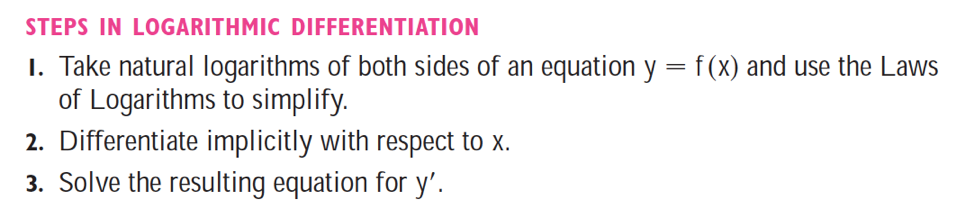
\includegraphics{fig1.png}
\end{figure}
\subsection*{Examples}
\begin{itemize}
    \item[(a)] Differentiate $y=\frac{x^{3/4}\sqrt{x^2+1}}{(3x+2)^5}$.\vspace{4cm}
    \item[(b)] Differentiate $f(x)=x^{\sqrt{x}}$.\vspace{4cm}
\end{itemize}
\begin{tcolorbox}
\subsection*{Definitions of $e$}
\begin{itemize}
    \item $\displaystyle e=\lim_{x\rightarrow 0}(1+x)^{1/x}$
    \item $\displaystyle e=\lim_{n\rightarrow \infty}\left(1+\frac{1}{n}\right)^n$
\end{itemize}
\end{tcolorbox}
\end{document}